\section{Inverses, Isomorphisms and determinants}
\subsection{Inverse}
\definition{Inverse function}{
    Let $T:U\to V$ be bijective.
    The \textbf{inverse of} $T$ is the unique function $T^{-1}$ that satisfies
    \begin{align*}
        T^{-1}(T(x))= x,\\
        T(T^{-1}(y))=y
    \end{align*}
    for all $x\in U, y\in V$.\\
    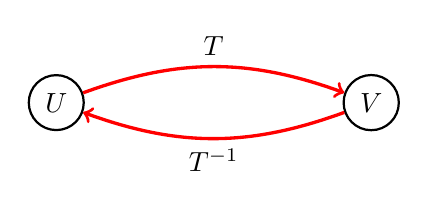
\begin{tikzpicture}
		\begin{scope}[every node/.style={circle,thick,draw}]
			\node (A) at (0,0) {$U$};
			\node (B) at (4,0) {$V$};
		\end{scope}
	
\begin{scope}[
	every edge/.style={draw=red,very thick}]
\path [->] (A) edge [bend left=20] node [above,midway]{$T$} (B);
\path [->] (B) edge [bend left=20]node [below,midway]{$T^{-1}$} (A);
\end{scope}
	\end{tikzpicture}
}
How do we know this inverse exists? We know that for each $y\in V$ there is exactly one
$x\in U$ that satisifes $T(x)=y$, so we can set $T^{-1}(y)$ to be this particular value of $x$ for each y.
This definition of the inverse sounds tautological, so let us apply this to linear transformations.
\proposition{
    Let $T:\reals^n\to\reals^n$ be a bijective linear transformation.
    Then $T^{-1}$ is a linear transformation.
}
\begin{proof}
    We want to show that for any $\vec{y}_1,\vec{y}_2\in\reals^n$, $c\in \reals$,
    $T^{-1}(\vec{y}_1+\vec{y}_2)=T^{-1}(\vec{y}_1)+T^{-1}(\vec{y}_2)$ and $T^{-1}(c\vec{y}_1)=cT^{-1}(\vec{y}_1)$.

    The trick to solving this is to use the definition for inverses and switch back and forth with $T$ and $T^{-1}$, and apply linearity of $T$.
    \begin{align*}
        T^{-1}(\vec{y}_1)+T^{-1}(\vec{y}_2) &= T^{-1}(T(T^{-1}(\vec{y}_1)+T^{-1}(\vec{y}_2)))\\
        &=T^{-1}(T(T^{-1}(\vec{y}_1))+T(T^{-1}(\vec{y}_2))) \textrm{ (as $T$ is linear)}\\
        &=T^{-1}(\vec{y}_1+\vec{y}_2).
    \end{align*}
    For scaling,\begin{align*}
        cT^{-1}(\vec{y}_1) &= T^{-1}(T(cT^{-1}(\vec{y_1})))\\
        &=T^{-1}(c(T(T^{-1}(\vec{y_1}))))\\
        &=T^{-1}(c\vec{y}_1).
    \end{align*}
\end{proof}
This means that the inverse of $T$ has a matrix representation.
If we write $T(\vec{x})=A\vec{x}$ for some matrix $A$,
then there is some matrix $B$ such that $AB=BA=I_n$.
\definition{Matrix Inverses}{
    Let $A\in M_{m\times n}(\reals)$. If there exists $X\in M_{n\times m}(\reals)$ such that
    \[
    XA=I_n,
    \]
    we call $X$ the \textbf{left inverse} of $A$.
    Similarly, if there exists $Y\in M_{n\times m}(\reals)$ such that
    \[
        AY=I_m,
    \]
    we call $Y$ the \textbf{right inverse} of $A$.
    If both the left and right inverses exist and are equal, then we say that $A$ is \textbf{invertible}, and denote $X=Y$ the \textbf{inverse} of $A$, written as $A^{-1}$.
}
\begin{remark}
    If $A$ has a left and right inverse, then the left and right inverses are equal. Indeed, we have for a left inverse $X$ and a right inverse $Y$ of $A$,\[
    X= X(I_m)= X(AY) = (XA)Y = (I_n)Y = Y.
    \]
\end{remark}
As we have already seen, only bijective linear transformations have inverses, so that means we have more to add to That One Theorem. We also see that being invertible implies having a left and right inverse, so might expect that having a left or right inverse corresponds to the columns being linearly independent or span $\reals^m$. 
\example{
    $A\in M_{m\times n}(\reals)$ having a left/right inverse indeed corresponds to the conditions that the columns are linearly independent and the columns span $\reals^m$. Figure out which conditions correspond to which.
}
There are two ways to think about this problem: one way is directly translate left and right inverses to the corresponding statements of the column vectors; the other way is to think of them in linear transformations and find out which one is surjective/injective. I will outline both methods.

\textbf{Method 1:} 
Without knowing where to go, let us suppose we want to prove $A$ has linearly independent columns and see which extra hypothesis we need. Suppose \[
    A\vec{x}=\vec{0}.
\]
We want to show $\vec{x} = \vec{0}$. This means we want to cancel the $A$ on the left, so we want to use the left inverse $X$. \[
\vec{x}=XA\vec{x} = X\vec{0} = \vec{0}.
\] 
So this means having a left inverse corresponds to linear independence.
Now to prove the columns of $A$ span $\reals^m$, we try to solve \[
A\vec{x}=\vec{b}
\] for any $\vec{b}\in\reals^m$.
To produce a solution $\vec{x}$ that can cancel $A$ from the right, we will need the right inverse $Y$, and set $\vec{x}=Y\vec{b}$, then
\[
A\vec{x}=AY\vec{b}=\vec{b}.
\]

\textbf{Method 2:}
We translate the problem into a linear transformation $T:\reals^n\to\reals^m$ being injective (linear independence) and surjective (span $\reals^m$).
Why does a left inverse imply injectivity? Let us suppose $T(\vec{x})=T(\vec{y})$, then the left inverse can immediately cancel out the $T$ from the left and give us $\vec{x}=\vec{y}$.

For surjectivity, let us break down the columns of the right inverse $Y=\begin{bmatrix}
    \vec{y}_1 & \ldots &\vec{y}_m
\end{bmatrix}$.
Then by the property of matrix multipication, we can consider each column to see \[
A\vec{y}_j = \vec{e}_j.
\]
Since the basis vectors can build anything in $\reals^m$, we can just use the corresponding linear combination of the $\vec{y}_j$'s to build anything in $\reals^m$.
This means we have three extra equivalences for a matrix being invertible.

\theorem{This/That One}{
    Let $A=[\vec{v}_1\ldots \vec{v}_n]\in M_{n\times n}(\reals)$, and $T:\reals^n\to\reals^n$ be the unique linear transformation satisfying $T(\vec{x})=A\vec{x}$ for all $\vec{x}\in\reals^n$.
	Then the following are equivalent.
	\begin{enumerate}
		\item $\{\vec{v}_n,\ldots,\vec{v}_n\}$ form a basis.
		\item $\{\vec{v}_n,\ldots,\vec{v}_n\}$ are linearly independent.
		\item $\{\vec{v}_n,\ldots,\vec{v}_n\}$ span $\reals^n$. \\ $\vdots$
	\end{enumerate}
	
	\begin{thatonethmlist}
		\item $A$ is invertible.
		\item $A$ as a left inverse.
		\item $A$ has a right inverse.
	\end{thatonethmlist}
}

Finally, we want to compute this inverse $A^{-1}$. Let us set the columns \[
A=[\vec{a}_1 \ \vec{a}_2 \ \ldots \ \vec{a}_n],\ 
A^{-1}=[\vec{b}_1 \ \vec{b}_2 \ \ldots \ \vec{b}_n],
\] 
then the condition $AA^{-1}=I_n$ translates to \begin{align*}
	A\vec{b}_1&=\vec{e}_1,\\
	A\vec{b}_2&=\vec{e}_2,\\
	&\vdots \\
	A\vec{b}_n&=\vec{e}_n.
\end{align*}
Which means we just have to solve $n$ different linear systems. We can do them all at once: by reducing the matrix \[
\begin{bmatrix}[cccc|cccc]
	\vec{a}_1 & \vec{a}_2 & \ldots &\vec{a}_n
	&\vec{b}_1 & \vec{b}_2 & \ldots &\vec{b}_n
\end{bmatrix}
\]
to rref,
we will get \[
\begin{bmatrix}[c|c]
	I_n & *
\end{bmatrix}
\]
if $A$ is invertible. The $*$ will be the solutions $\vec{b}_k$'s, which means $*$ is the inverse of $A$.

\subsection{Isomorphisms}
\definition{Isomorphism}{
	Let $T:U\to V$ be a bijective linear transformation. We call $T$ an \textbf{isomorphism} and the vector spaces $U$ and $V$ are \textbf{isomorphic}. We denote this $U\simeq V$.
}
Recall many sections ago, we said that many types of vector spaces are very similar to $\reals^n$. Now that we have defined isomorphic vector spaces, we have a concrete statement of what it means to be similar.
\theorem{Finite dimensional real vector spaces $\simeq \reals^n$ }{
Let $V$ be a finite dimensional real vector space. Then $V\simeq \reals^n$ for some $n\in\mathbb{N}$.
}
\begin{proof}
	Since $V$ is finite dimensional, let $\{v_1,...,v_k\}$ be a basis for $V$.
	We just need to construct an isomorphism from $\reals^n \to V$. What is an easy way to define this? We just need to define where each of the standard basis vectors $\vec{e}_j$ goes. This gives us a very natural choice to guess that the isomorphism $T:\reals^k\to V$ defined by \[
		T(\vec{e}_j)=v_j,	
	\]
	or equivalently \[
	T(\vec{x})=x_1v_1+x_2v_2+\ldots+x_kv_k
	\]
	is bijective. This is indeed bijective, which you have confirmed in a previous exercise.	
\end{proof}
\corollary{
	Let $V$ be finite dimensional. Then every basis of $V$ has the same number of vectors.
}
\begin{proof}
	Let $\{v_1,\ldots,v_k\}$ and ${w_1,\ldots, w_l}$ be two bases for $V$. Then by the construction in the previous theorem, we have $V\simeq \reals^k$ and $V\simeq \reals^l$. So $\reals^k\simeq \reals^l$ and thus $k=l$.
\end{proof}
\definition{Dimension of a vector space}{
	Let $V$ be finite dimensional. The \textbf{dimension} of $V$ is denoted dim$(V)$, and is the number $n$ for which $V\simeq \reals^n$.
}
\subsection*{Understanding generalized vector spaces}
We can use coordinates to understand finite dimensional vector spaces. Let $V$ be $n$-dimensional, and pick a basis $\{v_1,\ldots,v_n\}$ for $V$. Then each element $w\in V$ can be written as a \textit{unique linear combination} of the basis vectors, or \[
	v=c_1v_1+c_2v_2+\ldots+c_nv_n=\begin{bmatrix}
		v_1&v_2&\ldots&v_n
	\end{bmatrix}\begin{bmatrix}
		c_1\\c_2\\\vdots\\c_n
	\end{bmatrix}.
\]Therefore, we can make sense of linear transformations between finite dimensional spaces as transformations $\reals^n\to\reals^m$. To make this concrete, let dim$V=n$, dim $W=m$, and pick bases $\{v_1,\ldots,v_n\},\{w_1,\ldots,w_m\}$ for $V$ and $W$ respectively. Using our coordinate representation, for any transformation $T:V\to W$, we can pick a matrix representation of $\tilde{T}:\reals^n\to\reals^m$ such that the two paths from $\reals^n\to\reals^m$ lead to the same result

\begin{tikzpicture}
	\begin{scope}[every node/.style={circle,thick,draw}]
		\node (A) at (0,0) {$V$};
		\node (C) at (4,0) {$W$};
		\node (B) at (0,-4) {$\reals^n$};
		\node (D) at (4,-4) {$\reals^m$};
	\end{scope}
	\node [left of =B]{$\begin{bmatrix}
		c_1\\ \vdots \\ c_n
	\end{bmatrix}$};
	\node [right of =D]{$\begin{bmatrix}
		d_1\\ \vdots \\ d_m
	\end{bmatrix}$};
	\node [right of =C]{$w$};
	\node [left of =A]{$v$};
\begin{scope}[
every edge/.style={draw=red,very thick}]
\path [->] (B) edge node [left,midway]{coordinate representation of $V$} (A);
\path [->] (A) edge node [above,midway]{$T$} (C);
\path [->] (C) edge node [right,midway]{coordinate representation of $W$} (D);

\path [->,dotted] (B) edge node [above,midway]{ $\tilde{T}$} (D);
\end{scope}
\end{tikzpicture}\\
In particular, this correspondence of using coordinates is how we motivated the use of linear independence for computing the dimension of the span of vectors. If $v_1,\ldots,v_k$ are linearly independent, span$(v_1,\ldots,v_k)$ has a basis $\{v_1,\ldots,v_k\}$ and is isomorphic to $\reals^k$ using coordinates.
\subsection*{Rank Nullity Theorem}
Recall the Rank of a matrix is the number of pivots in its rref. 
\proposition{
	Let $A\in M_{n\times m}(\reals)$. Then\[
		\textrm{rank}(A)= \textrm{dim}(\textrm{col}(A))
	\]
}
The intuition behind this statement is as follows: If you take all the columns that has a pivot in the rref, you will get a linearly independent set of vectors. This statement says that the span of these vectors is exactly col$(A)$, so forms a basis for the column space.  
\begin{proof}
	We need to show two things: First, if we isolate the pivot columns, we have a linearly independent set of vectors. Next, we have to show the span of these vectors equals the column space of $A$.
	
	Let $S$ be a sequence of row operations that reduce $A$ to rref$(A)$.

	For linearly indepence, we isolate the columns of $A$ with pivot in rref$A$ to create a new matrix $A'$ of $n\times \textrm{rank}(A)$. The same sequence $S$ applied to $A'$ will reduce it to row echelon form, with a pivot in every column. Therefore, the vectors are linearly independent. 

	To show they span the column space, we want to show for each $\vec{b}$ that $A\vec{x}=\vec{b}$ has a solution, $A'\vec{y}=\vec{b}$ has a solution in $\vec{y}$. To show this, we see that applying $S$ to $
	\begin{bmatrix}[c|c]
		A &\vec{b}
	\end{bmatrix}
	$
	will give matrix in rref with no pivot in the final column. So applying $S$ to $\begin{bmatrix}[c|c]
		A' &\vec{b}
	\end{bmatrix}
	$
	will also lead to a matrix in rref with no pivot in the final column.
\end{proof}
Similarly, we can define a term for the dimension of nullspace of a matrix. \definition{Nullity}{
	Let $A\in M_{n\times m}(\reals)$. We define the \textbf{nullity} of $A$\[
	\textrm{Nullity}(A)=\textrm{dim}(N(A))
	\]
}
\proposition{
	$\textrm{Nullity}(A)$ is the number of columns in rref$(A)$ without pivots. 
}
We have a way to generate a basis for the nullspace, using the rows without a pivot, so this follows from the algorithm. 
Now we have rank corresponding to the columns with pivots and nullity corresponding to the columns without pivots. This means that for any $n\times m$ matrix, the sum of rank and nullity is always the number of columns $m$. This is the statement of the Rank-Nullity Theorem. 
\theorem{Rank-Nullity}{
	Let $A\in M_{n\times m}(\reals)$. Then \[
		\textrm{Rank}(A)+\textrm{Nullity}(A)=m.
	\]
	Phrased in terms of a linear transformation $T:U\to V$,
	\[
	\textrm{dim}(\textrm{Im}(T))+ \textrm{dim}(\textrm{ker}(T)) = \textrm{dim}(U).
	\]
} 

\subsection{Determinants}
We now move towards the last equivalence for That One Theorem. Recall in the intuition behind the \hyperref[thm:2.48]{Matrix Representation of Linear Transformations}, we constructed a grid and showed that a linear transformation is a change in the coordinate system.\\
\begin{figure}[h]
	\begin{subfigure}[l]{0.4\textwidth}
		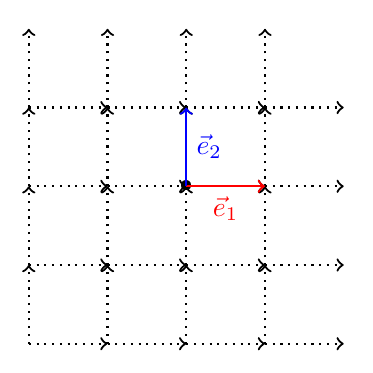
\begin{tikzpicture}
			\draw (0,0) node{\textbullet};
			\foreach \i in {-2,...,1}{
				\foreach \j in {-2,...,1}{
					\draw [->,thick,dotted] (\i,\j)--(\i+1,\j);
					
					\draw [->,thick,dotted] (\i,\j)--(\i,\j+1);
				}
			}
			\draw [->,color=red,thick] (0,0)--(1,0) node[midway, below]{$\vec{e}_1$} ;
			\draw [->,color=blue,thick] (0,0)--(0,1) node [right,midway]{$\vec{e}_2$};
			\end{tikzpicture}
			\caption{Original grid}
	\end{subfigure}
	\begin{subfigure}[r]{0.6\textwidth}
		\begin{tikzpicture}
			\draw (0,0) node{\textbullet};
			\foreach \i in {-1,...,1}{
				\foreach \j in {-1,...,1}{
					\draw [->,thick,dotted] (\i*2-\j,\j+\i)--(\i*2-\j+2,\i+\j+1);
					
					\draw [->,thick,dotted] (\i*2-\j,\j+\i)--(\i*2-\j-1,\i+\j+1);
				}
			}
			\draw [->,color=red,thick] (0,0)--(2,1) node[midway, below right ]{$T(\vec{e}_1)$} ;
			\draw [->,color=blue] (0,0)--(-1,1) node [above right ,midway,thick]{$T(\vec{e}_2)$};
			\end{tikzpicture}
			\caption{Transformed grid}
	\end{subfigure}
\end{figure}
The original grid squares become grid `parallelograms'. Indeed, if you extend to three dimensions, you can get grid `parallelepipeds'.
To say that the transformation is surjective means that the transformed unit square/cubes have non-zero area/volume and can thus tessellate.



\begin{figure}[h]
	\begin{subfigure}[l]{0.4\textwidth}
		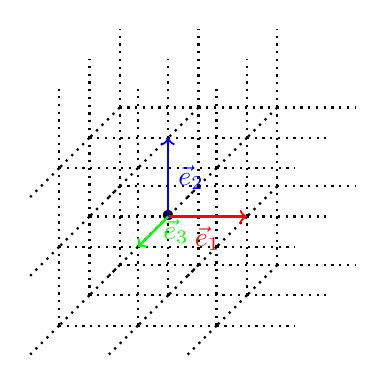
\begin{tikzpicture}
			\draw (0,0) node{\textbullet};
			\foreach \i in {-1,...,1}{
				\foreach \j in {-1,...,1}{
                    \foreach \k in {-1,...,1}{

					\draw [-,thick,dotted] (\i,\j,\k)--(\i+1,\j,\k);
					
					\draw [-,thick,dotted] (\i,\j,\k)--(\i,\j+1,\k);
					\draw [-,thick,dotted] (\i,\j,\k)--(\i,\j,\k+1);
                    }
				}
			}
			\draw [->,color=red,thick] (0,0,0)--(1,0,0) node[midway, below]{$\vec{e}_1$} ;
			\draw [->,color=blue,thick] (0,0,0)--(0,1,0) node [right,midway]{$\vec{e}_2$};
            \draw [->,color=green,thick] (0,0,0)--(0,0,1) node [right,midway]{$\vec{e}_3$};
			\end{tikzpicture}
			\caption{Original grid}
	\end{subfigure}
	\begin{subfigure}[r]{0.6\textwidth}
		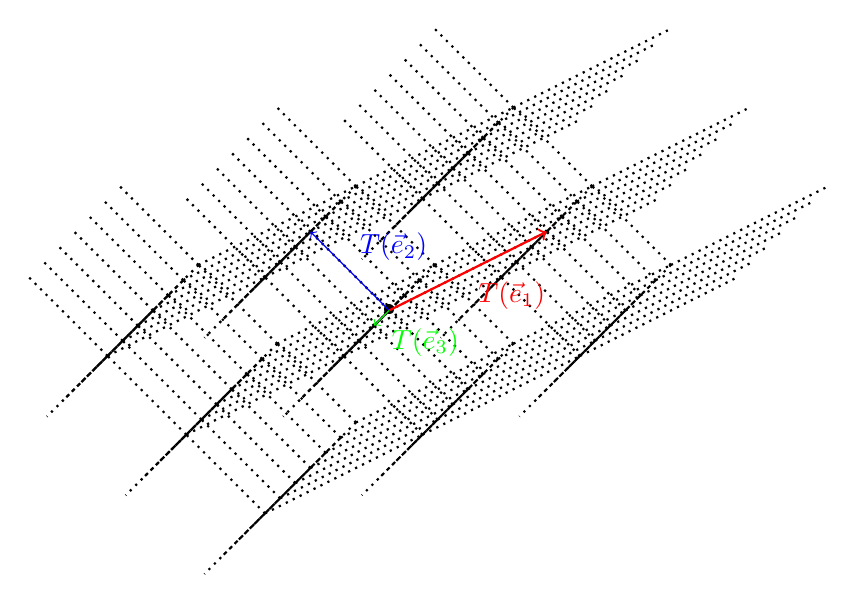
\begin{tikzpicture}
			\draw (0,0) node{\textbullet};
			\foreach \i in {-1,...,1}{
				\foreach \j in {-1,...,1}{
                    \foreach \k in {-3,...,3}{

					\draw [-,thick,dotted] (\i*2-\j,\j+\i,0.5*\k)--(\i*2-\j+2,\i+\j+1,0.5*\k);
					
					\draw [-,dotted,thick] (\i*2-\j,\j+\i,0.5*\k)--(\i*2-\j-1,\i+\j+1,0.5*\k);
					\draw [-,dotted,thick] (\i*2-\j,\j+\i,0.5*\k)--(\i*2-\j,\i+\j,0.5*\k+2);
                    }
				}
			}
			\draw [->,color=red,thick] (0,0)--(2,1) node[midway, below right ]{$T(\vec{e}_1)$} ;
			\draw [->,color=blue] (0,0)--(-1,1) node [above right ,midway,thick]{$T(\vec{e}_2)$};
			\draw [->,color=green] (0,0,0)--(0,0,0.5) node [below right,midway,thick]{$T(\vec{e}_3)$};
			\end{tikzpicture}
			\caption{Transformed grid}
	\end{subfigure}
    \caption{I tried my best, please use a bit of imagination}
\end{figure}
Here we use the god-given formula for the determinant.
\definition{Determinant}{
	We define a determinant function $\det : M_{n\times n}(\reals)\to\reals$ as follows.\begin{itemize}
		\item $\det [a] = a$ for a $1\times 1$ matrix $[a]$
		\item For higher dimensions $A = [a_{i,j}] \in M_{n\times n}(\reals)$, we recursively define \[
			\det A  = \sum_{i=1}^n (-1)^{i+j} a_{i,j} \det A_{i,j}
		\] for any $1\leq j\leq n$. Any value of $j$ will give the same formula upon expansion.
	\end{itemize}
}\begin{remark}
	$A_{i,j}$ is the the \textbf{minor} of the matrix $A$ where you delete the $i$-th row and $j$-th column.
	If \begin{align*}
	A&=\begin{bmatrix}
		a& b &*\\
		* & * & *\\
		c& d & *
	\end{bmatrix},\\
	A_{2,3}&=\begin{bmatrix}
		a&b\\c&d
	\end{bmatrix}.
	\end{align*} 
	
\end{remark}
\begin{remark}
	The recursive formula also works for 
	\[			\det A  = \sum_{i=1}^n (-1)^{i+j} a_{j,i} \det A_{j,i}
		\]
		where instead of expanding along the $j$-th row, we expand along the $j$-th column.
\end{remark}
\proposition{
	For small matrices, we have these simplified formulae.
	\begin{itemize}
		\item[$1\times 1$] $\det ([a])=a.$
		\item[$2\times 2$] $\det \left(\begin{bmatrix}
			a&b\\
			c&d
		\end{bmatrix}\right)=ad-bc$. 
		\item[$3\times 3$] $\det \left(\begin{bmatrix}
			a&b&c\\d&e&f\\g&h&i
		\end{bmatrix}\right)= aei+bfg+cdh-ceg-afh-bdi.$
	\end{itemize} 
}
\begin{remark}
	The mnenomic for memorizing the $3\times 3$ determinant is as follows:
	Extend the matrix as \[
	\begin{bmatrix}[ccc|cc]
		a&b&c&a&b\\d&e&f&d&e\\g&h&i&g&h
	\end{bmatrix}
	\]
	and take the difference between the red diagonal products and the blue diagonal products.
	\begin{figure}[h]
		\centering
		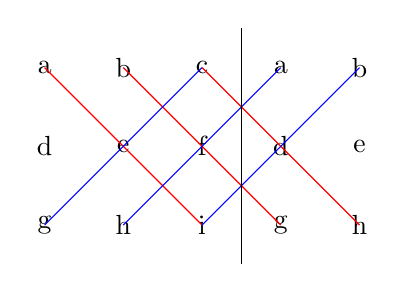
\begin{tikzpicture}
			\node (A) at (0,0) {a};
			\node (B) at (1,0) {b};
			\node (C) at (2,0) {c};
			\node (AA) at (3,0){a};
			\node (BB) at (4,0){b};
			\node (D) at (0,-1) {d};
			\node (E) at (1,-1 ){e};
			\node (F) at (2,-1){f};
			\node (DD) at (3,-1){d};
			\node (EE) at (4,-1){e};
			\node (G) at (0,-2) {g};
			\node (H) at (1,-2){h};
			\node (I) at (2,-2){i};
			\node (GG) at (3,-2){g};
			\node (HH) at (4,-2){h};
	
			\draw[-,color=red] (0,0)--(2,-2);
			\draw[-,color=red] (1,0)--(3,-2);
			\draw[-,color=red] (2,0)--(4,-2);
			\draw[-,color=blue] (2,0)--(0,-2);
			\draw[-,color=blue] (3,0)--(1,-2);
			\draw[-,color=blue] (4,0)--(2,-2);
			\draw[-,color=black] (2.5,0.5)--(2.5,-2.5);
		\end{tikzpicture}
	\end{figure}
	
\end{remark}
As you have seen in a previous chapter, the formula for the determinant of a $3\times 3$ matrix coincides with the volume of the parallelepiped spanned by the column vectors.


\example{
	Calculate the determinant of the rotational matrix \[
	R_\theta=
	\begin{bmatrix}
		\cos\theta &-\sin \theta \\
		\sin \theta&\cos \theta
	\end{bmatrix}\].
}
We just put this in the formula to get \[
	\det R = \cos^2\theta - (-\sin^2\theta) = \cos^2\theta + \sin^2\theta = 1
\]
regardles of the value of $\theta$.
\example{
	Calculate the determinant of an upper-triangular matrix in the form \[
	U=\begin{bmatrix}
		a_1& *& *&\ldots& *\\
		0 & a_2 & *& \ldots&*\\
		0&0&a_3& \ldots & * \\
		\vdots & & &\ddots& \\
		0 & 0 & 0 & \ldots & a_n
	\end{bmatrix}\in M_{n\times n}(\reals).
	\]
}
Let's consider the special case $n=3$. We do not know the values of $*$, but if we write out \[
	\begin{bmatrix}[ccc|cc]
		a_1&*&*&a_1&*\\0&a_2&*&0&a_2\\0&0&a_3&0&0
	\end{bmatrix},\]
the only diagonal that can possible have all non-zero entries gives the product $abc$. So the determinant of a triangular matrix is always the product of the diagonal terms.
The determinant of an upper triangular matrix is always the product of the diagonal terms. To show this, we need to exploit the recursive formula for the determinant.
If we expand along the first column, most of the terms in the sum are $0$, except the first term that gives \[
	(-1)^{1+1} a_1 \det \left( \begin{bmatrix}
		 a_2 & *& \ldots&*\\
		0&a_3& \ldots & * \\
		\vdots  & &\ddots& \\
		 0 & 0 & \ldots & a_n
	\end{bmatrix}\right),
\]
which is $a_1$ times the determinant of a smaller upper triangular matrix. If we know that this $(n-1)\times (n-1)$ matrix has determinant $a_2a_3\ldots a_n$, this will prove the formula for a $n\times n$ matrix, then this result will prove the formula for a $(n+1)\times (n+1)$ matrix and so on! This technique is known as Mathematical Induction. If you want to prove a statement is true for all natural numbers $n$, you can show that it is true when $n=1$, and show that if the statement is true for $n=k$, it is also true for $n=k+1$.
\begin{proof}
	We show that the determinant of $U$ is $(a_1\ldots a_n)$ by induction on the value of $n$.

	\textit{Base Case:} The determinant of the matrix $[a_1]$ is $a_1$, which is evidently the product of all the diagonal terms.
	
	\textit{Induction step:} Suppose the determinant of a $k\times k$ upper triangular matrix is the product of the diagonal terms. We compute the determinant of a $(k+1)\times (k+1)$ matrix in the form
	\begin{align*}
		U=[u_{i,j}]=\begin{bmatrix}
			a_1& *& *&\ldots& *\\
			0 & a_2 & *& \ldots&*\\
			0&0&a_3& \ldots & * \\
			\vdots & & &\ddots& \\
			0 & 0 & 0 & \ldots & a_{k+1}
		\end{bmatrix}.
	\end{align*}
	Applying the recursive formula and expanding along the first column, the only non-zero $u_{j,1}$ term is $u_{1,1}=a_1$, so \begin{align*}
		\det U &= (-1)^{1+1} a_1 \det \left( \begin{bmatrix}
			a_2 & *& \ldots&*\\
		   0&a_3& \ldots & * \\
		   \vdots  & &\ddots& \\
			0 & 0 & \ldots & a_{k+1}
	   \end{bmatrix}\right)\\
	   &= a_1 (a_2 a_3\ldots a_{k+1}) 
	\end{align*}
	by applying the hypothesis on the $k\times k$ upper triangular matrix. Then the determinant of a $(k+1)\times (k+1)$ matrix is the product of the diagonal terms. 
	By the Principle of Mathematical Induction, the determinant of an upper triangular matrix of any size is the product of its diagonal terms.
\end{proof}


\proposition{
	The elementary row operations change the determinant of a matrix in the following way:\begin{itemize}
		\item \textit{(Row Swap)} The determinant is multiplied by $-1$.
		\item \textit{(Scaling)} The determinant is multiplied by the scaling constant.
		\item \textit{(Sum)} The determinant does not change.  
	\end{itemize}
}
The proof of this is not very enlightening, so we will skip it. It boils down to working with the general determinant formula and doing intense algebra manipulation.

However, we have the following corollary 
\corollary{
	The determinant of a matrix can be computed as follows:\begin{enumerate}
		\item Reduce the matrix to rref (or row echelon form).
		\item Take the product of the diagonal terms.
		\item Multiply this product by $1/c$ for every time you scaled a row by $c$ in computing the rref.
		\item Multiply this product by $-1$ for every time you swaped two rows in computing the rref.
		\item The final product is the determinant of the matrix.
	\end{enumerate}
}
\theorem{This/That One (Determinants)}{

Let $A=[\vec{v}_1\ldots \vec{v}_n]\in M_{n\times n}(\reals)$, and $T:\reals^n\to\reals^n$ be the unique linear transformation satisfying $T(\vec{x})=A\vec{x}$ for all $\vec{x}\in\reals^n$.
	Then the following are equivalent.
	\begin{enumerate}
		\item $\{\vec{v}_n,\ldots,\vec{v}_n\}$ form a basis.
		\item $\{\vec{v}_n,\ldots,\vec{v}_n\}$ are linearly independent.
		\item $\{\vec{v}_n,\ldots,\vec{v}_n\}$ span $\reals^n$. \\$\vdots$
	\end{enumerate}
	
	\begin{thatonethmlist}
		\item $\det A \neq 0.$ 
	\end{thatonethmlist}
}
\begin{proof}
	Recall the motivation for introducing the determinant is the signed n-dimensional volume of the paralellotope formed by the column vectors. If (and only if) the volume is non-zero, they can tesselate the whole $\reals^n$ space.

	To show the equivalence of det$A\neq 0$, we can use the condition from That One Theorem that rref$(A)=I_n$, and the previous corollary for computing determinants. If the determinant is $0$, then the product of the diagonal terms of rref$A$ has a zero, so rref$(A)\neq I_n$. On the converse, if the determinant is non-zero, all the diagonal terms in rref$(A)$ are non-zero. The only way this can happen for a matrix in rref is when the matrix is also the identity matrix.
\end{proof}
\theorem{Determinant of Product is Product of Determinant}{
	Let $A,B\in M_{n\times n}(\reals)$, then \[
	\det(AB)=\det (A) \det(B)
	\]
}
\begin{proof}
	First we consider the case where $\det (A)=0$. By That One theorem, the column space of $A$ is not $\reals^n$. Let $\vec{v}\notin \textrm{col}(A)$. Then $\vec{v}\notin \textrm{col} (AB)$. So by That One Theorem again $\det (AB)=0$.
	
	Now we can let $\det (A)\neq 0$. By That One Theorem, we have a sequence of row opeations transforming $A\to I_n$. Denoting the row operations as matrices, we have $X_1,\ldots,X_k\in M_{n\times n}(\reals)$ such that\[
	X_k \ldots X_1A=I_n,
	\]
	so \[
		X_k \ldots X_1AB =I_nB=B,
	\]
	or that the same row operations turn $AB$ into $B$. Starting with $\det (B)$, we can reverse the row operations (and scaling according to the factors in \hyperref[prop:2.75]{corollary 2.76}) to get $\det(AB)=\det(A)\det(B)$.
\end{proof}
\exercises
\begin{exerciselist}
	\item Compute the determinants of the following matrices: (you may find row reduction helpful) \begin{enumerate}
		\item $\begin{bmatrix}
			1&1&2\\1&3&5\\6&4&1
		\end{bmatrix}$
		\item $\begin{bmatrix}
			1&2&3&4\\2&1&4&3\\1&4&2&3\\4&3&2&1
		\end{bmatrix}$
		\item $\begin{bmatrix}
			0&0&0&0&3\\
			1&0&0&0&2\\
			0&1&0&0&1\\
			0&0&1&0&4\\
			0&0&0&1&2\\
		\end{bmatrix}$
		\item $\begin{bmatrix}
			0&x&y\\-x&0&z\\-y&-z&0
		\end{bmatrix}$
	\end{enumerate}
	\item For a $2\times 2$ matrix $\begin{bmatrix}
		a&b\\c&d
	\end{bmatrix}$, show that the matrix is invertible when $ad-bc$ is non-zero, and its inverse in this case is given by \[
	\begin{bmatrix}
		a&b\\c&d
	\end{bmatrix}^{-1}=
	\frac{1}{ad-bc}\begin{bmatrix}
		d & -b\\-c& a
	\end{bmatrix}.
	\]
	\item Let $A=[a_{i,j}]\in M_{n\times n}(\reals)$. The \textbf{transpose} of $A$ is denoted $A^T$ and has entries $b_{i,j}=a_{j_i}$ i.e. you swap the rows and columns, as an example \[
	\begin{bmatrix}
		1&2&3\\0&2&3\\0&0&3
	\end{bmatrix}^T=\begin{bmatrix}
		1&0&0\\2&2&0\\3&3&3
	\end{bmatrix}
	\]
	Show that det$(A)=$det$(A^T)$, thus $A$ is invertible if and only if $A^T$ is invertible.
\end{exerciselist}
\newpage
As a wrapup, here is That One Theorem with the things we have proven so far. (There are a few more you will encounter in Spring Quarter.)
\theorem{This/That One}{
	Let $A=[\vec{v}_1\ldots \vec{v}_n]\in M_{n\times n}(\reals)$, and $T:\reals^n\to\reals^n$ be the unique linear transformation satisfying $T(\vec{x})=A\vec{x}$ for all $\vec{x}\in\reals^n$.
	Then the following are equivalent.
	\begin{enumerate}
		\item $\{\vec{v}_n,\ldots,\vec{v}_n\}$ form a basis.
		\item $\{\vec{v}_n,\ldots,\vec{v}_n\}$ are linearly independent.
		\item $\{\vec{v}_n,\ldots,\vec{v}_n\}$ span $\reals^n$.
		
		\item The system of equations $A\vec{x}=\vec{b}$ has exactly one solution for each $\vec{b}\in\reals^n$.
		\item The system of equations $A\vec{x}=\vec{b}$ has at most one solution for each $\vec{b}
		\in\reals^n$.
		\item The system of equations $A\vec{x}=\vec{b}$ has at least one solution for each $\vec{b}\in\reals^n$.
		\item rref$(A)=I_n.$
		\item rref$(A)$ has a pivot in every column.
		\item rref$(A)$ has a pivot in every row.
		\item Rank$(A)=n$.
		\item $N(A)=\{\vec{0}\}$.
		\item col$(A)=\reals^n$.
		\item $T$ is bijective.
		\item $T$ is injective.
		\item $T$ is surjective.
		\item $\textrm{ker}(T)=\{\vec{0}\}.$
		\item $\textrm{Im}(T)=\reals^n$.
		\item $A$ is invertible.
		\item $A$ as a left inverse.
		\item $A$ has a right inverse.
		\item $\det A \neq 0.$
		\item $\det A^T \neq 0.$ 
	\end{enumerate}
}
\section{End of Chapter Exercises}
\begin{exerciselist}
	\item Let $\vec{v}_1,\vec{v}_2,\ldots,\vec{v}_k\in \reals^n$ be non-zero and pairwise orthogonal. That is $\vec{v}_i\cdot\vec{v}_{j}=0$ if $i\neq j$ and $>0$ if $i=j$. \begin{enumerate} [label=(\alph*)]
		\item Show that $\vec{v}_1,\ldots,\vec{v}_k$ are linearly independent. (Hint: what happens when you take the dot product of $c_1\vec{v}_1+\ldots+c_k\vec{v}_k=\vec{0}$ with $\vec{v}_1$ on both sides?)
		\item Show that $k\leq n$.
		\item Now suppose $k=n$. Find an inverse for the matrix \[
		[\vec{v}_1 \ \ldots \ \vec{v}_n]. 
		\]
		Consider computing left and right inverses, one way is significantly harder than the other.
	\end{enumerate}
	\item Recall the \textbf{transpose} of $A=[a_{i,j}]\in M_{n\times m}(\reals)$ is an $m\times n$ matrix denoted $A^T$ and has entries $b_{i,j}=a_{j_i}$. \begin{enumerate}[label=(\alph*)]
		\item Show that for any $\vec{x}\in \reals^m, \vec{y}\in \reals^n$, $A\vec{x}\cdot \vec{y}=\vec{x}\cdot \vec{y}.$
		\item Show that for two matrices $A,B$,  $(AB)^T=B^T A^T$, whenever the product $AB$ is defined.
		\item Conclude that if $A$ has an inverse, $(A^T)^{-1}=(A^{-1})^T.$
	\end{enumerate}
	
	\item Let $\vec{x}\in \reals^3$, $A\in M_{3\times 3}(\reals).$ Suppose $A^2\vec{x}\neq\vec{0}$ and $A^3\vec{x}=\vec{0}$. Show that $\vec{x}, A\vec{x},A^2\vec{x}$ span $\reals^3$.
	\item Let $A\in M_{n\times n}(\reals)$
	\begin{enumerate}[label=(\alph*)]
		\item Show that the solutions of the equation \[
			A\vec{v}=\lambda \vec{v}
			\]form a subspace of $\reals^n$ for any value $\lambda$.
		\item Show that this subspace is not the trivial subspace if and only if \[
		\textrm{det}(A-\lambda I_n)=0.
		\]
		\item Conclude that if $n$ is odd, there is some non-zero vector $\vec{v}$ such that $A\vec{v}$ is parallel to $\vec{v}$. You may use the fact that all odd-degree polynomials $p(x)$ have a real root, which you can prove using the intermediate value theorem considering the values of $\lim_{x\to \infty}p(x)$ and $\lim_{x\to -\infty}p(x)$. 
		\item Suppose $\lambda_1,\ldots,\lambda_k$ are all distinct and $\vec{v}_1,\ldots,\vec{v}_k\in \reals^n$ non-zero vectors such that $A\vec{v}_j=\lambda_j\vec{v}_j$ for all $j$. Show that $\vec{v}_1,\ldots ,\vec{v}_k$ are linearly independent, thus $k\leq n$. You might it helpful to consider $k=1$ then apply induction.
		\item Consider the sum \[
		S=\sum_{\lambda\in\reals} \textrm{Nullity}(A-\lambda I_n).
		\]
		The previous part shows that at most $n$ values of $\lambda$ have a non-zero nullity, so we can make sense of the infinite sum as the sum over the finite number of values of $\lambda$ for which the nullspace is non-trivial. Show that $S\leq n$.
	\end{enumerate}
\end{exerciselist}
